% !TEX root = ../tfg.tex

\section{Motivación y antecedentes}
\label{sec:motivacion}

% IDEAS (borrar antes de pasar la memoria al tutor)
% - El problema: analizar el pádel; el paso siguiente, que nadie ha dado, es
%   clasificar el tipo de golpe.
% - El hueco, dicho con precisión («hasta donde se ha podido comprobar»): no hay
%   trabajos publicados ni herramientas abiertas que clasifiquen el tipo de golpe
%   a partir del vídeo. Matices: Cartes Domínguez (2023) lo clasifica con una
%   pulsera de sensores, no con vídeo; hay aplicaciones comerciales (aiball,
%   Padelytics, Padel AI) que no publican ni su método ni su precisión. El
%   estado del arte lo respalda.

\section{Objetivos generales y específicos}
\label{sec:objetivos}

% IDEAS (borrar antes de pasar la memoria al tutor)
% - En prosa y con conectores, no en lista («En primer lugar se quiso…»).
% - Para quién: clubes que quieran este análisis y tengan, o pongan, una cámara
%   fija al fondo de la pista, en alto.
% - General: que esos clubes tengan una herramienta de análisis de nivel
%   profesional para mejorar.
% - Listón: que funcione lo bastante bien para usarse de verdad, no una cifra
%   fijada de antemano.
% - Específicos: detectar el instante de cada golpe; identificar al jugador;
%   clasificar el tipo (derecha, revés, remate, saque); el visor (estadísticas
%   por jugador: golpes por tipo, total, mapa de calor; saltar al instante de
%   cada golpe; que sea útil).
% - El tipo no va solo: sin cuándo y quién no hay estadísticas por jugador.
%   Cadena; la pieza nueva es la última.
% - Decorte et al., base del cuándo y el quién: no reinventar un método que
%   funcionaba; compararse solo para comprobar la reimplementación.
% - No son objetivos: los datos etiquetados (medio: no existían con el tipo; se
%   cuentan en Datos); la evaluación por torneos (va en Experimentos).
% - Alcance, al final y en pocas frases: fuera el marcador y el resultado;
%   bandeja, víbora y dejada; cámaras móviles o a ras de pista; partidos
%   completos (trabaja por puntos); saber quién es cada jugador entre puntos.
%   Evaluado con retransmisiones (las grabaciones anotadas de que se dispone,
%   cumplen la condición de cámara); otras alturas = trabajo futuro (PADELVIC,
%   cuatro alturas).
% - Para Descripción informática o Datos (no para aquí): entra el punto ya
%   cortado, con audio y sin anotar, y la pista se marca a mano una vez por
%   cámara (cuatro esquinas y extremos de la red); sale, por cada golpe,
%   instante, jugador y tipo; todo golpe recibe uno de los cuatro tipos (sin
%   «sin clasificar»; un 7 % de los etiquetados no es ninguno); los tipos se
%   agrupan por gesto (volea de derecha = derecha); J1-J4 son posiciones dentro
%   del punto (J1-J2 al fondo), no personas. Posible: por qué es difícil.
% - Figura: figuras/problema.pdf (scripts/build_problem_figure.py). VIGO_14
%   (Danish Padel Open), revés de J3 a 4,52 s, con los modelos entregados, que
%   vieron este punto al entrenar: ilustra la salida, no demuestra el acierto;
%   los modelos entrenados sin VIGO también aciertan este golpe. Pie: solo el
%   torneo (CVSPORTS se cita en Datos). Se puede mover a donde encaje mejor.

\begin{figure}[htbp]
  \centering
  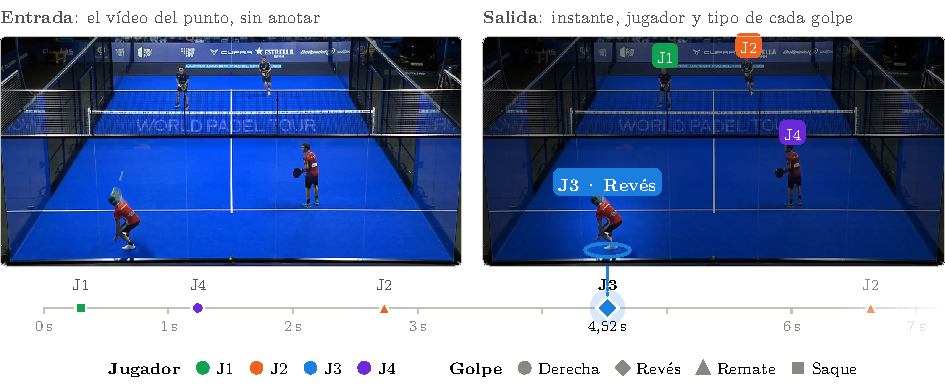
\includegraphics{figuras/problema}
  \caption{Un punto antes y después de procesarlo (Danish Padel Open 2023).}
  \label{fig:problema}
\end{figure}

\section{Metodología del trabajo}
\label{sec:metodologia}
